\documentclass{ou-report-vaf}

% Dit template is gemaakt door P.J. Molijn in het kader van zijn afstuderen aan de OU in 2014.
% Waarvoor hartelijk dank.
% Minieme maar belangrijke wijzigingen zijn aangebracht door E.M. van Doorn
% Het template is versimpeld door Sylvia Stuurman, 2019.
% Het template is aangepast voor de ba informatica door Harrie Passier, Tanja Vos en Pekka Aho 2020 
% Het tamplate is aangepast met nieuwe huisstyle door Rick Neeft, 2021

\def\mytitle{How can automated comparison of inferred models help testers finding bugs?}
\def\myauthor{Rick Neeft}
\def\myStudentId{851829973}
\def\myPresentationDate{T.B.D. 2022}

\newcommand{\testar}{\textsc{testar }}
\newcommand{\testarnet}{\textsc{testar .NET }}

\begin{document}

    \pagenumbering{roman}

    % Elements of the thesis
    %%%% TITLE PAGE %%%%%%%
% front cover should be a empty as possible. Title (subtitle) - Name - student Id and thesis presentation date

%to prevent that the title page will be referred as page 1, 
%which will give the warning that there is a page 1 twice.

\pagestyle{plain}

\begin{titlepage}
    \newgeometry{right=100pt,left=58.8pt}

    \pagecolor{ou-light-gray}
    \afterpage{\nopagecolor}
    
    %% Insert the OU logo at the top right corner of the page
    %% PowerPoint contains 84 pt margin in picture
    \begin{tikzpicture}[remember picture,overlay]
                \node at (current page.north east)[anchor=north east,inner sep=58.8pt]{
            
\includegraphics[scale=0.5]{images/ou-text-logo.png}
        };
    \end{tikzpicture}
    
    %% Extra whitespace at the top.
    \vspace*{5\bigskipamount}
    
    %% add title without hypens
    \nohyphens{{\color{ou-red}\Huge\bf \mytitle}}
     
    \bigskip
    %{\large subtitle, if any}
    
    %\bigskip \bigskip
    %by
    \bigskip \bigskip
    
    {\Large\bf \myauthor}\\
    {\large\myStudentId}
    
    {\myPresentationDate}
    
\end{titlepage}

% reset geometry since we changed them for the title page
\newgeometry{right=0.875in,left=.875in}

%%%% END TITLE PAGE %%%%%%%
    
    % Page 2 must be left blank
    \myemptypage
    
    % Page 3 contains all compulsory data.
    \addcontentsline{toc}{chapter}{Compulsory data}

\myauthor, \myStudentId\\
\textbf{\mytitle}\\
\myPresentationDate
\vspace*{\fill}

Open University of the Netherlands, Faculty of Science\\
Master's Programme in Software Engineering\\
\\
Graduation committee

Chair: Prof. Dr. Tanja E.J. Vos\\
Primary supervisor: Dr. Pekka Aho\\
Seconday supervisor: Fernando Pastor Ricós

Course code: IM9906
\newpage
    
    % Acknowledgements
    %\chapter*{Acknowledgements}
\addcontentsline{toc}{chapter}{Acknowledgements}

I want to thank my supervisors, Pekka Aho, Fernando Pastor Ricós and Tanja Vos, for the opportunity and support of my graduation project. The weekly meeting and feedback were always inspiring and gave me good directions on what to do. I am grateful for allowing me to develop the application in C\#. Besides academic learning, using C\# and Blazor is extremely helpful in my day-to-day career.

Thanks to WithSecure, especially Joona Oikarinen and Tatu Aalto, for their input and feedback regarding the Analysis website and the docker setup.

I want to thank my wife for her support and for allowing me to sit in our home office for countless hours. 

Thank you to my family, and special thanks to my mother, who always supported me and pushed me to achieve my life goals. 

Last but not least, I want to thank my employer, VECOZO, for providing me with time and resources to finish my Masters. 

Rick Neeft\\
\myPresentationDate
    %\myemptypage
    
    % Table of contents
    \begingroup
        \hypersetup{linkcolor=black}
        \tableofcontents
    \endgroup
    \newpage
    
    % Summary
    %\chapter*{Summary}
\addcontentsline{toc}{chapter}{Summary}
lorem ipsum blah blah yadda yadda yadda
    %\newpage
    
    % the content of the thesis
    \pagenumbering{arabic}
    
    \chapter{Introduction} \label{introduction}
    
Regression testing is considered a good practice when testing new software versions before being released to the general public. 
However, due to shortened release cycles, the time to market has decreased drastically. As a result, software test teams have less time to test all new software features, let alone try all other elements to prevent unwanted side effects \cite{rapid-release-cycle-issues}.
The research proposed aims to apply change detection between two versions of the GUI of the system under test. 

This section introduces the proposed research discussing the background and context, followed by the research problem, research aims, research questions and why this research is important.

\section{Background}
The TESTAR tool solves a significant obstacle when it comes to testing the GUI. With TESTAR, the tester can automatically start testing the GUI without any upfront scripts. TESTAR automatically generates and executes test sequences based on elements derived from the GUI \cite{VosAho2021}. In recent master graduation assignments, TESTAR has been extended with an inferred model generation module \cite{thesisMulders}, and it became easier to integrate TESTAR in build and release pipelines in a DevOps environment \cite{thesisSlomp}. Those two additions make it easier to run TESTAR upon each source code integration and retrieving an inferred model about the GUI. In a proof of concept, two inferred models are compared to get changes between versions of the SUT \cite{stateDiff}.

Some companies might write down changes of the software in a changelog. However, some changelogs might not be complete and unwanted side effects might be missing entirely. Comparing two inferred models shows all the changes between versions of a SUT, even the unwanted ones.

\section{Research problem}
Although the proof of concept for change detection is a good start, it lacks some basic functionality. For example, it compares calculated abstract hashes with each other. As a result, even the slightest change in GUI results in a removed and added state between versions.

In addition to change detection, the change visualisation does not use the build-in visualisation tool. The proof of concept generates an HTML-based report, making it difficult to see where the change can be found and which steps the tester needs to take to navigate to the changed state in the software.

\section{The aim of the research}
The research aims to apply change detection on the inferred model created with the automated GUI testing tool TESTAR and research whether the outcome is helping testers finding bugs quicker. The main research questions are:

\begin{questions}
    \item How to detect changes between two versions of the SUT?
	\item How to visualise the detected differences to the user? 
\item How to validate the results of \ref{rq:detect-changes} and \ref{rq:diff-visualisation}?
\end{questions}

\section{Scope}
The scope of the research is change detection in GUI inferred models created by TESTAR. Researching how to make models and making significant changes to the creation of models are omitted. However, tweaking the model generation, like adding data that is not saved at the moment, and configuring TESTAR to create a good model, are in scope.

\section{Contribution}
When change detection is available in TESTAR, it becomes easy for testers to run the comparison in a continuous integration environment and receive an overview of the changes found in an updated version of the software.

As a side effect, the comparison and visualisation solutions can run outside the context of TESTAR and can be deployed to a docker environment.

\section{Document outline}
This research proposal is structured as follows. In section \ref{intoduction} the context, aim and objectives for this research proposal are introduced, together with the limitations for the expected outcome. Section \ref{background} describes the background of this proposal and contains knowledge that is available but might not be known by the readers. Section \ref{releatedWork} includes an overview of the material that can be seen as a direct foundation for this proposal or work that influences the expected outcome. Section \ref{questions} formulates the research questions for the thesis. The last section \ref{planning} will outline the chosen approach and planning for the graduation assignment.
    \newpage
    
    \chapter{Related Work}

%% TODO make better introduction for the chapter. 

\section{Background} \label{background}
This section describes the background of this proposal and contains information that is available but might not be known by students and readers. 

\subsection{Introduction into GUI Testing}
Ever since the first line of software is written, testers are testing its workings. While in the early day of software, the \acrfull{ui} was mainly terminals based or a set of blinking LEDs \cite{altair8800} \footnote{For example the ALTAIR 8800 computer \cite{altair8800}}, today we have an ever-increasing amount of \acrfull{gui} applications. Testings a GUI application is labour intensive and costs a lot of money \cite{gui-history}.

Initially, testers were using \acrfull{cr} software to automate their work. A tester would record a test scenario into the CR software, and then the CR software will execute the test case when needed. Using CR software, the time required to retest software decreases; however, the big downside is that when software changes, so must the recorded scripts \cite{gui-history}.

Then came \acrfull{mbgt}. With MBGT, the GUI elements and behaviour are abstracted on a higher level. The created models are used to generate abstract test cases. Those abstract test cases need to be mapped or transformed to get concrete test cases that are executed on the SUT. The downside of MBGT is the effort required to create the models and the need to have formal modelling expertise. Formal modelling expertise is not needed with the latest evolution in test automation: model inference. 

The \emph{model inference}, also known as model extraction and GUI Ripping \cite{gui-ripping}, is the current state-of-the-art approach to automate GUI testing \cite{gui-history}. Inferred models are state graphs based on the GUI of the SUT. There are two ways to generate inferred models; the first is a static approach where the source code of the  SUT is used to create a GUI model. The second is a dynamic approach where the GUI state is captured and extracted while being executed. 

The static approach has several downsides. First, the source code must be available, which is not always the case and secondly, it is challenging to capture behaviour based on the GUI source code. For example, with HTML, it is easy to generate a model; however, its behaviour is either in Javascript or server code.  It is possible to overcome those stumbling blocks by executing the SUT.
    
As for the Dynamic approach, it captures the model during test execution. The automated test tool interacts with the SUT in a scriptless and random way. This random scriptless approach is called \emph{Monkey testing}. Usually, test monkeys have no idea in which state the SUT is in and what type of input is allowed. It is therefore essential to make the test monkey smarter. A "smart test monkey" can be achieved by making them "see" the UI elements (Section \ref{data-retrieval}). Section \ref{testar-testauto} will give more details about how TESTAR is using smart test monkeys.

\subsection{What is TESTAR?} \label{what-is-testar}
TESTAR - or TEST* - is an automated software testing tool for the GUI level \cite{testar-about}. TESTAR started within the context of the \acrfull{fittest} project. TESTAR is open-source, the source code is published on GitHub \footnote{ \url{https://github.com/TESTARtool/TESTAR\_dev}}. A screenshot of the TESTAR tool is displayed in Figure \ref{fig:testar}.

\bigskip
\begingroup
\captionsetup{type=figure}
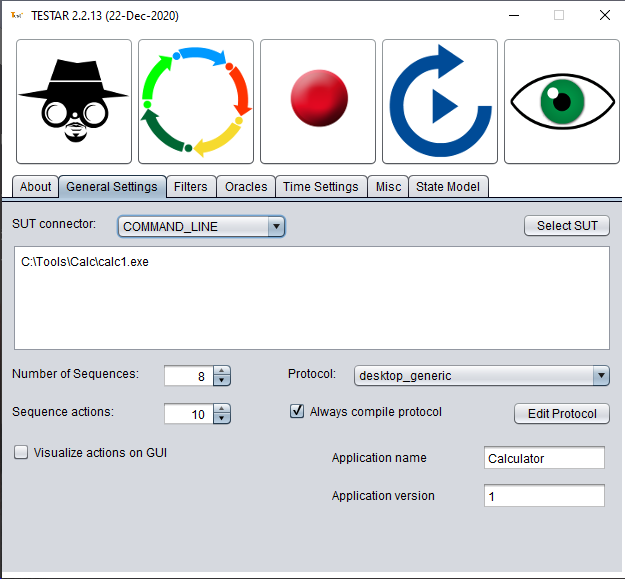
\includegraphics[scale=0.5]{images/testar.png}
\captionof{figure}{Screenshot of the TESTAR tool}\label{fig:testar}
\endgroup

TESTAR has several \emph{execution modes} in which it interacts with the SUT \cite{testar-manual}. From left to right, in figure \ref{fig:testar}, those are Spy, Generate, Record, Replay and View mode.

The \emph{Spy} mode allows the user to inspect a SUT and analyse how TESTAR is interpreting the widgets on the screen. Figure \ref{fig:calc-spy} shows the Windows calculator in spy mode. Dots on the GUI indicate actions that TESTAR could execute to interact with the SUT. Furthermore, within TESTAR, it is possible to filter out actions. Then, TESTAR will not execute those actions. The filtered actions are marked with a grey-coloured dot. A list with properties about the widget is shown when hovering, as well as a unique identifier of the current \emph{state}, more information about the state and the unique identifier can be found at section \ref{gui-state}.\par

\bigskip
\begingroup
\captionsetup{type=figure}
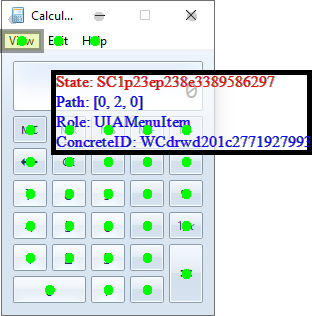
\includegraphics{images/calc-state.png}
\captionof{figure}{Screenshot of the Calculator with TESTAR Spy}\label{fig:calc-spy}
\endgroup

In the \emph{Generate} mode, TESTAR will start testing the specified system. Section \ref{testar-testauto} gives more details about TESTAR test automation.

The \emph{Record} mode allows a tester to record a test sequence manually. In the \emph{Replay} mode, existing test execution can be re-executed and lastly, the \emph{View} mode allows existing test executions to be viewed.

\newpage
\subsubsection{TEST automation} \label{testar-testauto}
TESTAR works without test scripts. Instead, it uses GUI Ripping and Monkey testing techniques. \emph{GUI Ripping}, first introduced by Memon et al. \cite{gui-ripping}, is a process to obtain the GUI's structure and execution behaviour automatically. As for \emph{Monkey testing}, it is a process in which decisions (interactions with the GUI) are randomly made. Section \ref{data-retrieval} will give more insights into GUI Ripping.

TESTAR is using a flow to execute tests on the SUT. This flow is as follows:
\begin{samepage}
\begin{enumerate}
    \item Start the SUT
    \item Scan the GUI and obtain the state (Section \ref{gui-state})
    \item Finding and selecting an action to execute
    \item Evaluate state with a test oracle (Section \ref{test-oracles})
    \item Stop the SUT when no actions are left to be executed or restart the SUT when more sequences are required.
\end{enumerate}
\end{samepage}

\bigskip
\begingroup
\captionsetup{type=figure}
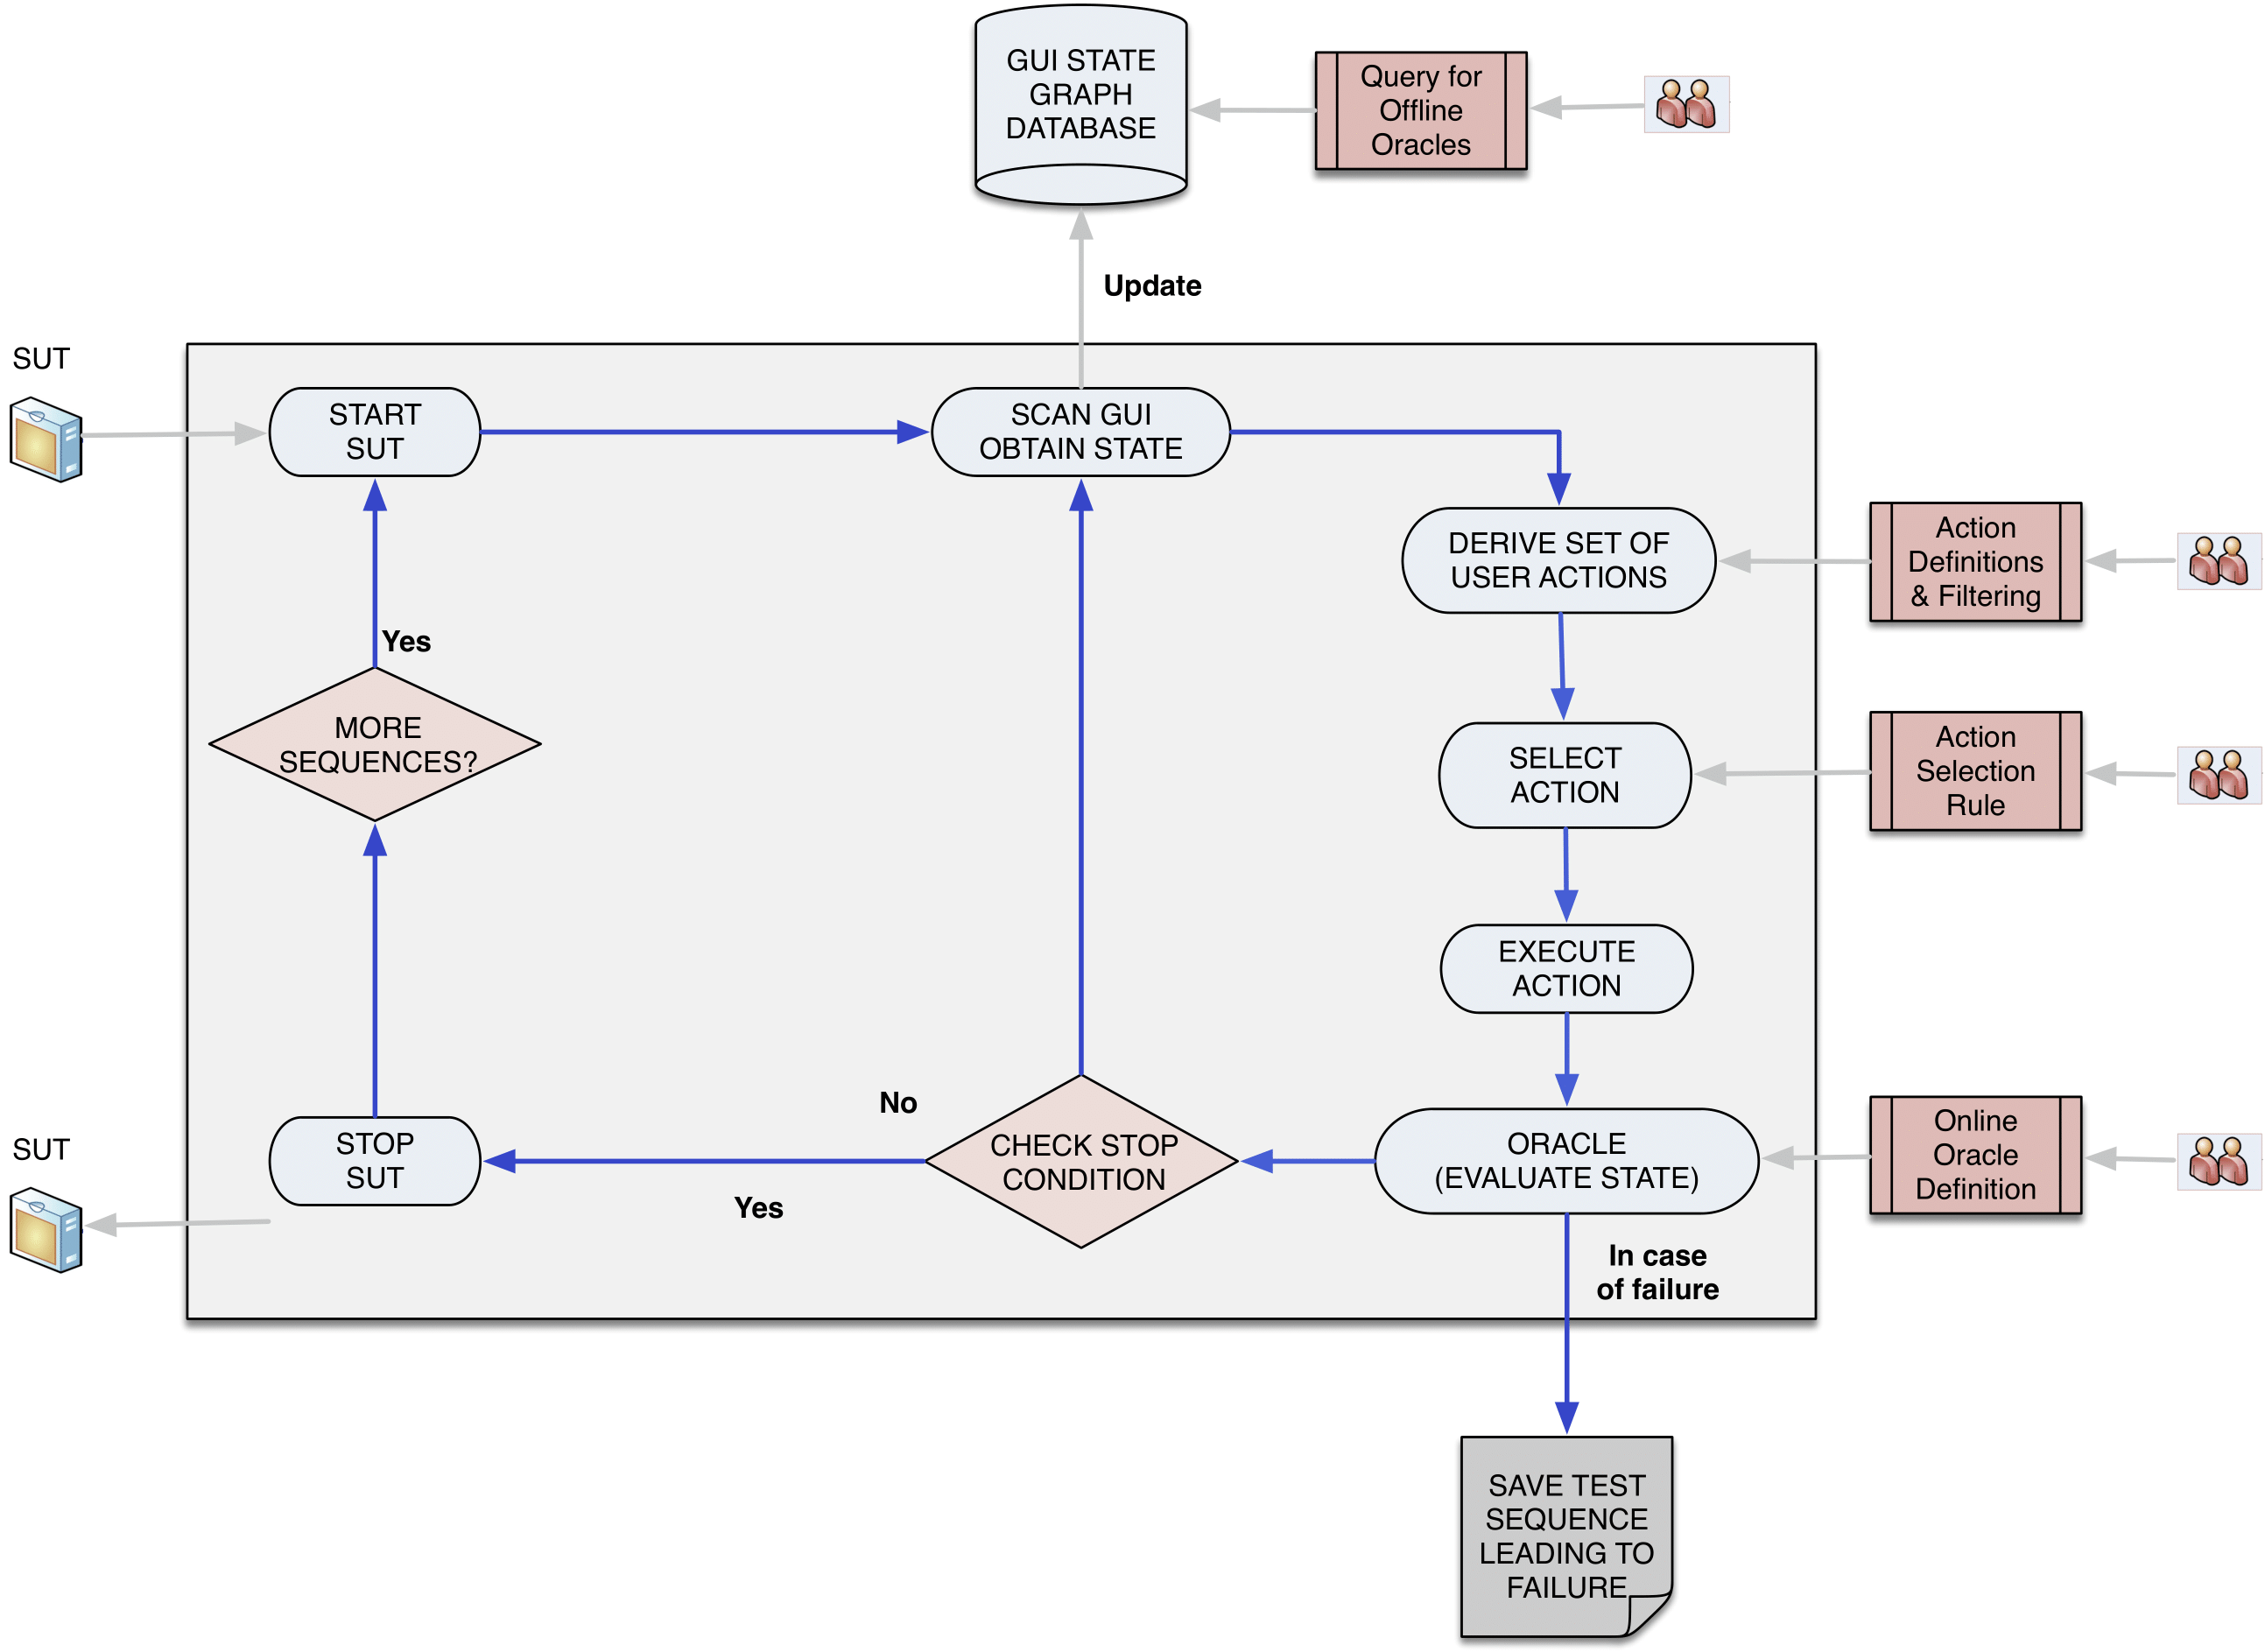
\includegraphics[scale=0.36]{images/testar-test-cycle.png}
\captionof{figure}{TESTAR test cycle \cite{testar-presentation}}\label{fig:testar-test-cycle}
\endgroup

Figure \ref{fig:testar-test-cycle} shows the flow graphically \cite{VosAho2021}. The test specialist needs to provide SUT details to TESTAR, like which actions should not be executed, and devise a mechanism that defines which SUT behaviour is correct and which is not, named a test oracle (Section \ref{test-oracles}). 

\subsection{How is the SUT tested} \label{test-oracles}
When software is tested, a method is needed to check the correct behaviour of the SUT. The method of checking is formally known as a \emph{test oracle} \cite{testOracles}. 

Outside the TESTAR context, an example of a test oracle could be a \emph{assertion} in software code. An assertion is a boolean expression created in a program by a software developer which checks the program's behaviour during run-time \cite{barr2014oracle}. Assertions can also be used in unit tests as displayed below on Listing \ref{code:assert}. 

%% do not indent code since it indents its extra in the LaTeX output
\begin{lstlisting}[language=Java, caption=Example assertion, label=code:assert]
@Test
public void testAdd(){
    Calculator sut = new Calculator();

    int expected = 3;
    int actual = sut.Add(1,2);

    Assert.assertEquals(expected, actual);
}
\end{lstlisting}

TESTAR comes with some test oracles out-of-the-box. Without any configuration, TESTAR will recognize crashes and unresponsiveness. It is also able to validate the GUI state with suspicious text. For example, a test sequence will fail when the title of a widget contains the word 'exception'. The input for the suspicious text is a regular expression that can be adjusted by the TESTAR user \cite{VosAho2021}. 

\subsubsection{Online and Offline Test oracles}
Test oracles come in two variants, \emph{online} or \emph{on-the-fly} test oracles and \emph{offline} test oracles \cite{VosAho2021}. With online test oracles, the state under test is being asserted for any anomalies during test execution. For example,  an online test oracle inspects the URL to check for any information being exposed in the query string. Offline test oracles will look into stored data - like logs - to find anomalies after test execution. For example, offline test oracles can inspect all the visited URLs to check for any exposed information in the query strings.

The two test oracle variants are complementary to each other and can run side by side. However, each variant comes with its strengths and weaknesses. The online test oracle takes up computation time because it inspects the state during test execution. This inspection of state slows down the test execution and may become an issue with time-critical SUTs. On the other hand, some issues - like the SUT becoming unresponsive - can only be checked during test execution. An offline test oracle is inspecting the gathered data after test execution has finished. Especially with larger data sets, this can become helpful. Inspecting the data may run in parallel, which can speed up the test oracle. Additionally, when developers create new offline test oracles, they can inspect the recorded data instead of executing a new test run \cite{de2019offline}.

\subsection{How is data retrieved} \label{data-retrieval}

Section \ref{testar-testauto} discussed how TESTAR is using GUI ripping to obtain the GUI's structure. A GUI consists of a non-empty set of UI components, known as \emph{widgets}. Examples of widgets are Windows or buttons; more examples can be found in Table \ref{tables:widgets} \cite{VosAho2021}. 

\begingroup
\captionsetup{type=table}
\begin{tabularx}{\textwidth}{ 
  | >{\raggedright\arraybackslash}X 
  | >{\raggedright\arraybackslash}X 
  | >{\raggedright\arraybackslash}X | }
    \hline
    Windows & Menus & Controls \\
    \hline
    \hline
    main windows & menu bars & buttons \\
    child windows & dropdown menus & textboxes \\
    popup windows & context-aware menus & links \\
    && radio buttons \\
    && checkboxes\\
    && dropdown select boxes\\
    && sliders\\
    && tabs\\
    && scrollbars \\
    \hline
\end{tabularx}
\captionof{table}{Example of GUI widgets \cite{VosAho2021}}\label{tables:widgets}
\endgroup

The widgets are structured hierarchically in a \emph{widget tree}. Each node in the tree is a widget with its related properties, such as the title, position and role. In figure \ref{fig:widget-tree} a compact widget tree is shown for the calculator. 

\bigskip
\begingroup
\captionsetup{type=figure}
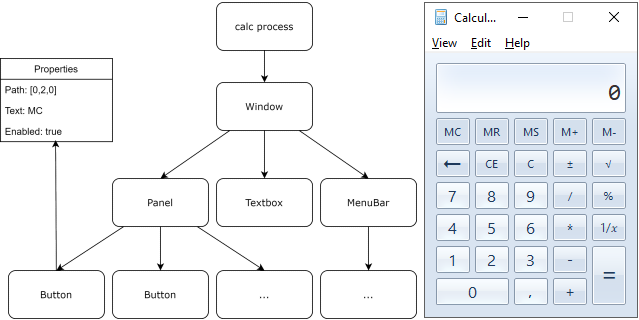
\includegraphics[scale=0.7]{images/calc-tree.png}
\captionof{figure}{A compact version of a widget tree for the calculator.}\label{fig:widget-tree}
\endgroup

\subsection{Widget data API}

In order to retrieve data from a SUT, TESTAR is making use of external APIs to access widgets that are part of the GUI \cite{thesisMulders}. TESTAR is using three different APIs.

In order to test a desktop application, TESTAR makes use of the Windows Automation API. The purpose of the Windows Automation API is to expose rich information about UI elements\cite{win-api-info}. For web applications, TESTAR uses Selenium Chromedriver. The Chromedriver is a tool for automated testing. It provides capabilities for navigating through web pages, user input, and JavaScript execution \cite{chrome-driver-info}. The latest API that TESTAR is using is Appium. Appium is a test automation tool for native, mobile web, and hybrid applications on iOS mobile, Android mobile, and Windows platforms \cite{appium-info}.

\subsection{GUI State} \label{gui-state}
In the previous sections, the widget tree is discussed and how the widgets are retrieved. In the widget tree, all the GUI elements with their properties are captured. The widget tree represents the state of the GUI when it has stopped executing any action. The GUI is at 'rest'. When an action is executed, the GUI can change, going to a new state. In figure \ref{fig:state-actions} the state change is represented in a small graph. 
\bigskip
\begingroup
\captionsetup{type=figure}
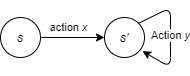
\includegraphics{images/state-action.png}
\captionof{figure}{An graph with two states and two actions.}\label{fig:state-actions}
\endgroup

The graph is a directed graph since every action changes the GUI from one state to the other. An action may lead to the same state, see figure \ref{fig:state-actions} action \textit{y}. However, that would mean that the action does not do anything or TESTAR does not indicate a change. For example, the GUI changes but not the property corresponding to the change is not included in the widget tree.

The universe of states and actions of the SUT's GUI makes up an inferred model. More information about the inferred model and how they are created can be found in section \ref{inferred-model}.

\subsection{How is data persisted}

TESTAR is using a database to store and retrieve state model data. Gier and Kager investigated which data storing solution would be beneficial to TESTAR \cite{GierKager}. The data solution must comply with six requirements. Generally speaking, the requirements were as follows: an open-source graph database with a straightforward query mechanism. The conclusion was that OrientDB was the best solution that met all the requirements.

\begin{samepage}
OrientDB is a Multi-Model NoSQL \acrfull{dbms} that combines four models \cite{orientDbModeling}:

\begin{itemize}
    \item \hyperlink{db:key-value}{Key/Value}
    \item \hyperlink{db:document}{Document}
    \item \hyperlink{db:graph}{Graph}
    \item \hyperlink{db:object}{Object}
\end{itemize}
\end{samepage}

A \hypertarget{db:key-value}{\emph{Key/Value}} is the simplest model and allows storing information (value) that is accessible with a key. Key/Values can be grouped into \textit{buckets}. However, OrientDB supports richer models in the form of document and graph elements.

A \hypertarget{db:document}{\emph{document}} is a schema-less set of key/value pairs. The \emph{key} allows access to the corresponding value. OrientDB allows the developer to store documents into \emph{clusters}. Relations between document are either embedded into other document or \emph{linked} to each other. Someone familiar with relational databases can view a cluster as tables, a document as the row and the key/value pairs are columns.

The \hypertarget{db:graph}{\emph{graph}} is a model consisting of \emph{Vertices} and \emph{Edges}. Vertices are the nodes in the graph, and the edge is the link between those nodes. In TESTAR terminology, a vertex represents state, and the edge is an 'action' from one state to the next. A Vertex consists of three elements: a unique identifier, a set with incoming Edges and outgoing Edges. An edge consists of four elements: a unique identifier, an incoming vertex (\emph{head}), an outgoing vertex (\emph{tail}) and a label that describes the relationship between the head and tail vertex.\par

The last model is the \hypertarget{db:object}{\emph{object}} that supports inheritance, like in the Object-Oriented programming paradigm.\par

Despite being a NoSQL database, OrientDB does support SQL as a query language \cite{sql-lang} albeit that it does not support all SQL statements. The majority of developers have experience with SQL \cite{sql-stats}, and as a result, new developers and students can start querying the TESTAR data and start expanding its features.\par

In addition to TESTAR, other applications can query the state model data in the OrientDB database as well. For example, developers and students can create external tools for a single purpose, like a state model difference application. When building external tools, the TESTAR application can be kept small and focus upon one objective: testing GUI applications. 

\section{Related work} \label{releatedWork}
This section covers an overview of the material that is the direct foundation for this research proposal.

\subsection{Inferred model} \label{inferred-model}
The master thesis by Mulders had two significant outcomes. The first is an inferred model module, and the second is the visualisation of the inferred models \cite{thesisMulders}. The visualisation model is a web-based application that shows the inferred model with screenshots and properties. Although the visualisation module becomes required when we want to visualise the result of the change-detection software, it is not necessary to go into depth in this document. This section will discuss what an inferred model is and how they are generated. 

The GUI state was discussed in section \ref{gui-state}. The section ended with the sentence that the universe of states and actions of the SUT's GUI makes up the inferred model. The inferred model is a directed graph showing the GUI-state of the application and the transactions between states. The vertex of the graph represents the GUI-state. Each vertex has a set of incoming and outgoing edges, called the actions. 

Figure \ref{fig:state-model} shows the result of the inferred model in the visualisation module.

\bigskip
\begingroup
\captionsetup{type=figure}
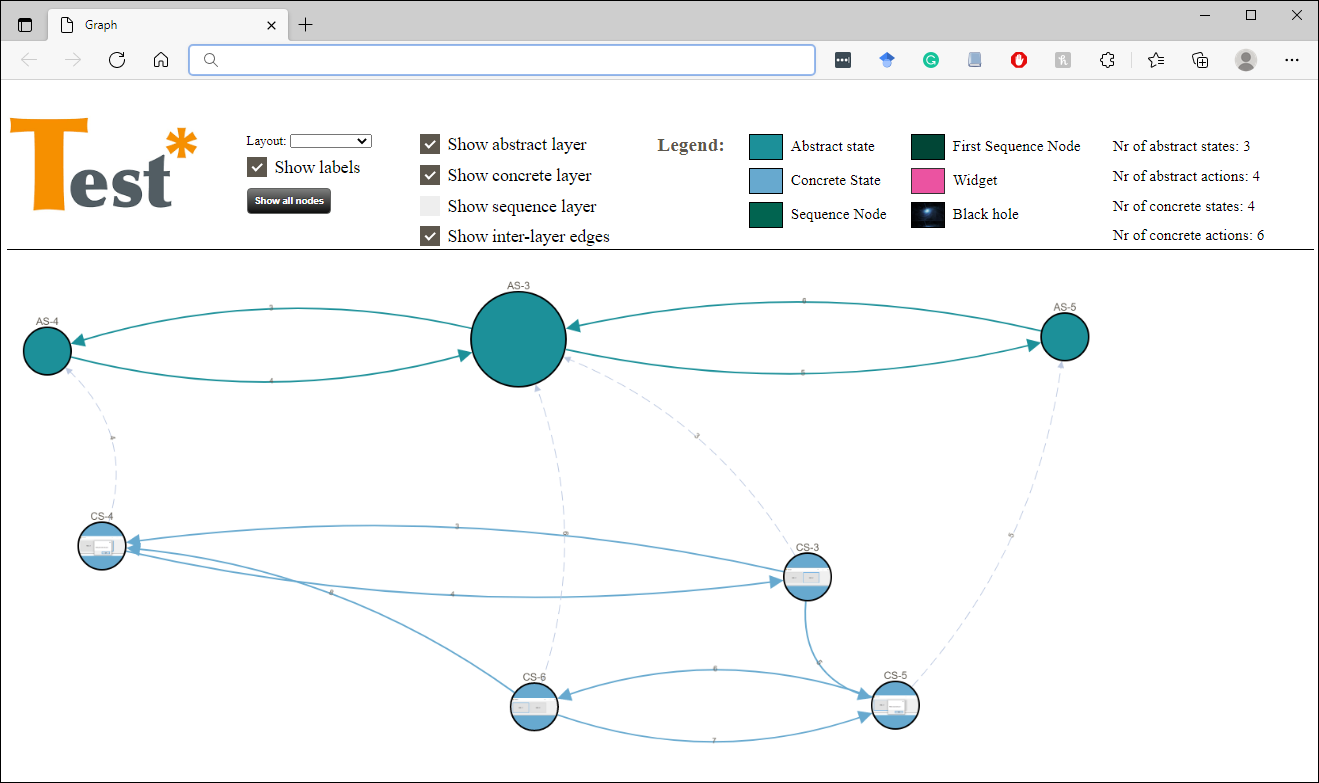
\includegraphics[scale=0.38]{images/state-model.png}
\captionof{figure}{an inferred model in the visualisation application}\label{fig:state-model}
\endgroup

In figure \ref{fig:state-model} two models can be observed. The first model, indicated by the AS text, shows the abstract model. The second, indicated by the CS text, shows the concrete GUI states. 

\subsubsection{Concrete model}
The concrete model contains all the data that could be retrieved from the GUI. The identification key uses a hash calculated over all the properties. Aside from the widget's properties, the concrete models also contain a screenshot of the GUI for each state \cite{thesisMulders}.

Figure \ref{fig:concrete-node} shows an example of a node in the concrete model. Upon selecting a node, the properties of the node show, including the screenshot taken during the test. The grey dotted line, indicated with the letter 'a', shows the connection with the abstract node, see section \ref{abstract-model} and figure \ref{fig:abstract-model} for more details. The two outgoing edges, indicated with the letter 'b', shows the two actions available in this state. The incoming edge, indicated with the letter 'c', shows how the state was reached. 

\bigskip
\begingroup
\captionsetup{type=figure}
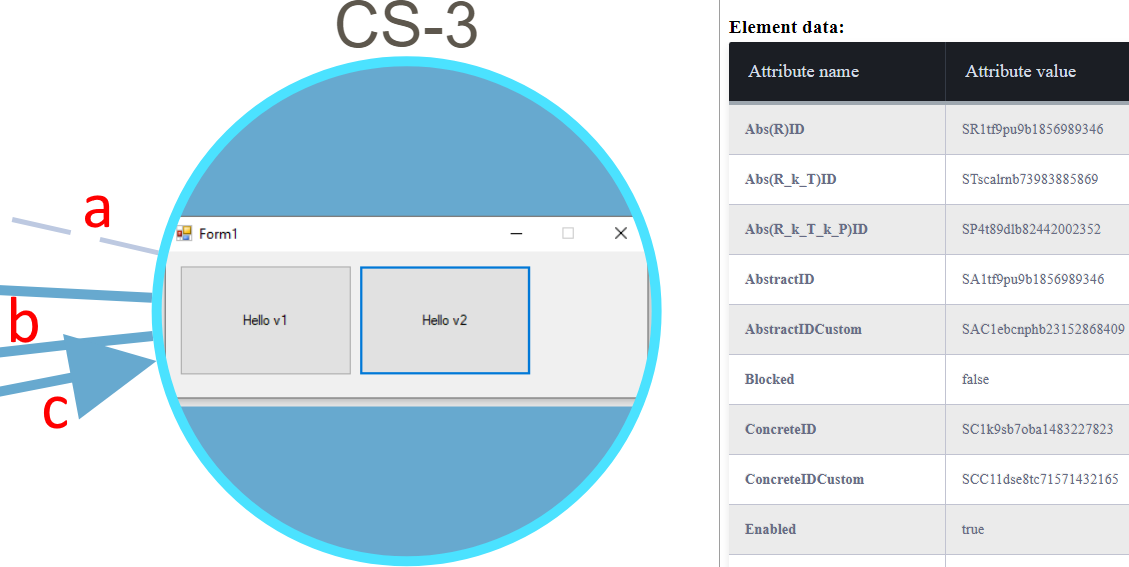
\includegraphics[scale=0.5]{images/concrete-model.png}
\captionof{figure}{A node from the concrete model}\label{fig:concrete-node}
\endgroup

\newpage
\subsubsection{Abstract model} \label{abstract-model}
Since the concrete models containing all the data from a GUI-state, they can become quite large.  Therefore an abstraction model is made \cite{thesisMulders}. Figure \ref{fig:abstract-model} shows an example of such a abstract node. The grey lines (from CS-3, CS-6 to AS-3) indicates which concrete state is abstracted. The properties of the abstract node are displayed, what the identifier is and which concrete state(s) it represents.

\bigskip
\begingroup
\captionsetup{type=figure}
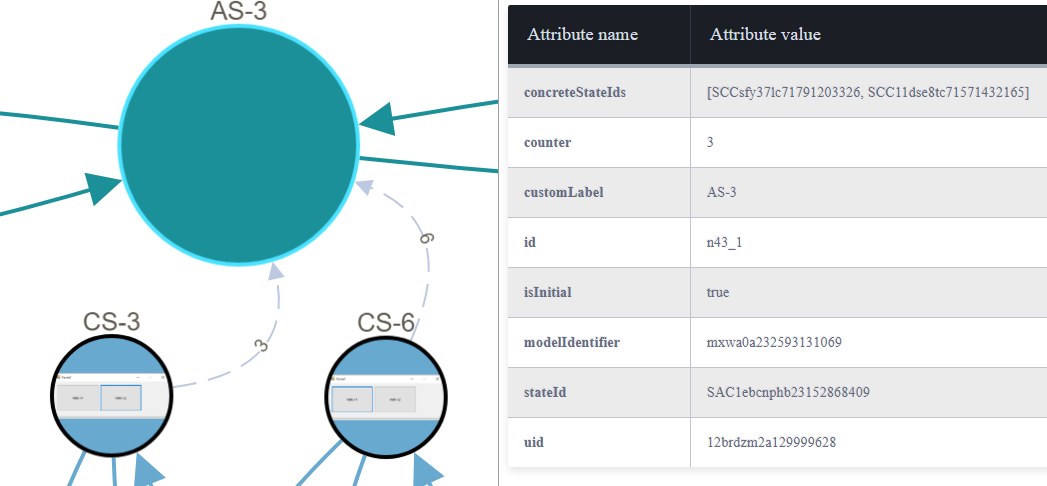
\includegraphics[scale=0.5]{images/abstract-model.png}
\captionof{figure}{A node from the abstract model}\label{fig:abstract-model}
\endgroup

\subsubsection{State identifiers} \label{state-identifiers}
Every state must have a unique id for identification. The identifier is calculated with the data from the widget tree. 

TESTAR uses a hashing algorithm that works as follows: the widgets' properties are concatenated and hashed. The outcome will be used as the identifier for a widget. The hashes from the widget in the widget tree are then combined and hashed to create an identifier for the GUI state \cite{VosAho2021}. The TESTAR's algorithm is similar to how a Merkle tree works, more information can be found at section \ref{merkle-tree}.

To identify the state (and actions), TESTAR calculates two state identifiers; an abstract and concrete state identifier. For the concrete state identifier, all the properties of a widget are used. For the abstract identifier, a subset of the properties is used. It is configurable which properties are used for the abstract identifier. By default the properties \textit{role}, \textit{title}, \textit{position} and \textit{enabled} are utilised \cite{VosAho2021, thesisMulders}.

When running TESTAR, it is possible to configure which widget properties should be used for the abstract state identifier. Figure \ref{fig:advance} shows the selection dialogue in which the user can select the properties for the abstract identifier.

\subsection{Merkle tree} \label{merkle-tree}
A Merkle tree is a hash tree data structure where a hash can identify each vertex. \cite{merkle-tree} The cryptographic hash is calculated by taking the hashes of the descendant vertices, combining them, and calculating a new hash from the combination. 

As written in the previous section (\ref{state-identifiers}), TESTAR's way of calculating the identification id for a widget or a GUI state is similar to that of the Merkle tree vertex. The hashed id for a widget is based on the hashed property values. Figure \ref{fig:merkle-tree} shows an example of a Merkle tree about how the GUI state identification id is calculated. The corresponding widget tree (Figure \ref{fig:widget-tree}), where the Merkle tree is based, is shown in the top right corner.

Although a Merkle tree usually is a binary tree \cite{merkle-tree}, having more than two descendant vertices is not considered a problem since the same Merkle-tree principle can be applied.

\bigskip
\begingroup
\captionsetup{type=figure}
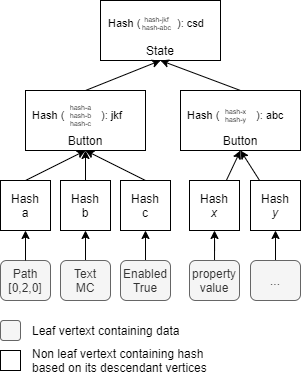
\includegraphics[scale=0.8]{images/merkle-tree-example.png}
\captionof{figure}{An short Merkle tree example based on a widget tree}\label{fig:merkle-tree}
\endgroup

\subsubsection{How is an inferred model created?}
This research focuses itself on the outcome of the obtain step as illustrated in figure \ref{fig:obtain-state-graph}, which is the top right part of figure \ref{fig:testar-test-cycle}.

\bigskip
\begingroup
\captionsetup{type=figure}
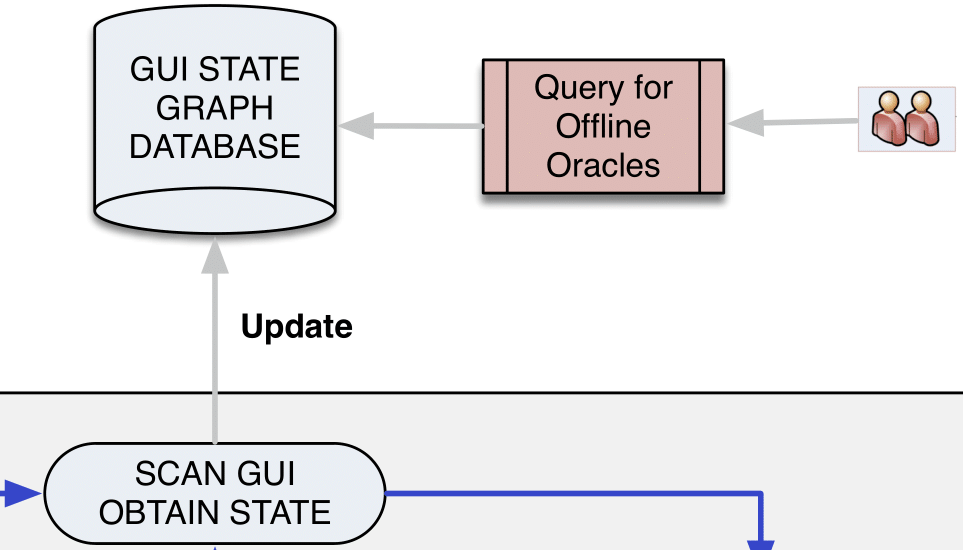
\includegraphics[scale=0.4]{images/obtain-state-graph.png}
\captionof{figure}{The focus of this research proposal \cite{testar-presentation}}\label{fig:obtain-state-graph}
\endgroup

Generating the inferred model starts when TESTAR start testing the SUT. After an action has been executed successfully, the state of the GUI is sent to the inferred model module. When the state is reached without action, it is marked as the initial state. 

The inferred model module generates the abstract and concrete state's and saves those in the model. The model is persisted in the OrientDb database. At last, a deterministic model check is being performed and saved \cite{testar-code}.

\subsection{State model difference}
The \verb|StateModel.Difference| package, added by Pastor Ricós\cite{stateDiff}, offers a proof of concept for calculating differences between the inferred state models. For the comparison, the \verb|abstractStateId| is used. 

Pastor Ricós difference algorithm\cite{stateDiff} outputs two classification of changes between two models: added and removed state. Let $A$ be a set of \verb|abstractStateId|s of version 1 of the SUT, and let $B$ be a set of \verb|abstractStateId|s of version 2 of the SUT. The removed states can be written as
\[A-B = \lbrace x | x \in A \wedge x \notin B \rbrace\]
the states that are added can be written as
\[B-A = \lbrace x | x \in B \wedge x \notin A \rbrace\]

\begingroup
\captionsetup{type=figure}
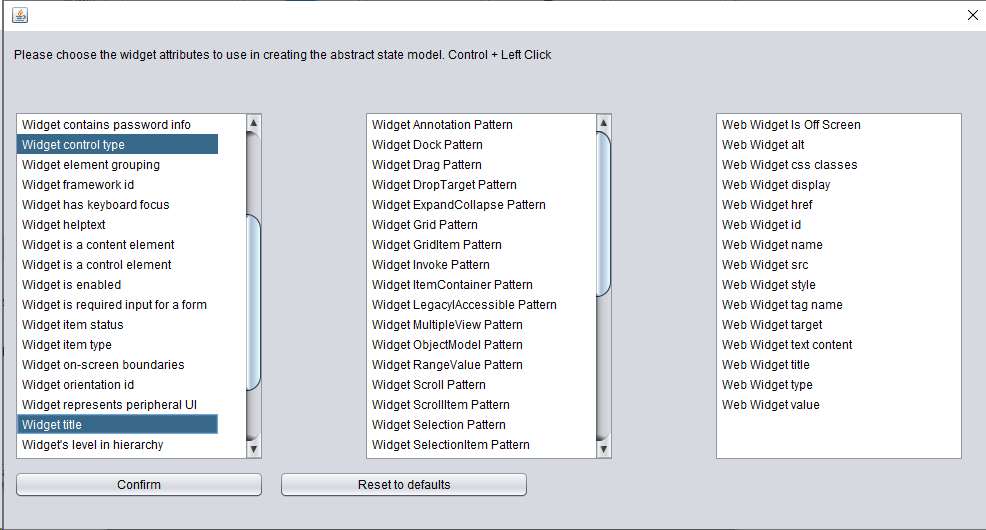
\includegraphics[scale=0.5]{images/attributes-state-model.png}
\captionof{figure}{Select widgets attributes for the abstractStateId}\label{fig:advance}
\endgroup

Using the \verb|abstractStateId| is excellent for the proof of concept and preliminary change detection, 
However, its boolean nature in which state exists or not can result in many 'false' changes. For example, when a widget is moved, the change detection should result in an altered state, not a removed and added state. 

Section \ref{state-identifiers} discussed how identifiers are generated, since the differences are calculated based on the \verb|abstractStateId| selecting the correct widget attributes is vital. Choosing too few attributes could result in conflicting differences like the same actions are removed and added. Choosing too many attributes could trigger a change in even the tiniest detail. Choosing the widget attributes can be done with the 'Advance' screen under the State model tab. See Figure \ref{fig:advance}.

For the research proposal, an experiment application is created; the two-buttons app. With the two-buttons app, it was possible to experiment with various TESTAR settings. The application is shown in figures \ref{fig:exp-v1}, \ref{fig:exp-v2} and \ref{fig:exp-v3}. As one can observe, the differences between version 1 and version 2 are the added button with the label 'Hello v2' and between version 2 and 3 the buttons' colour and position. 

\begin{tabularx}{\textwidth}{@{} 
   >{\raggedright\arraybackslash}X
   >{\raggedright\arraybackslash}X  }
    \begingroup
    \captionsetup{type=figure}
    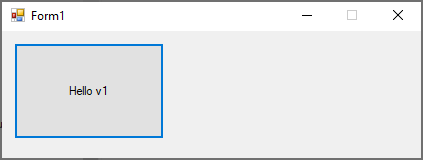
\includegraphics[scale=0.60]{images/exp-v1.png}
    \captionof{figure}{Version 1 of the experiment application}\label{fig:exp-v1}
    \endgroup
    &
    \begingroup
    \captionsetup{type=figure}
    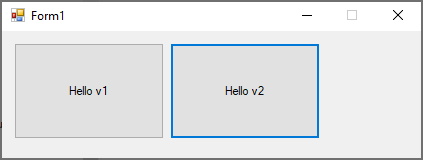
\includegraphics[scale=0.60]{images/exp-v2.png}
    \captionof{figure}{Version 2 of the experiment application}\label{fig:exp-v2}
    \endgroup
    
    \\
    
    \begingroup
    \captionsetup{type=figure}
    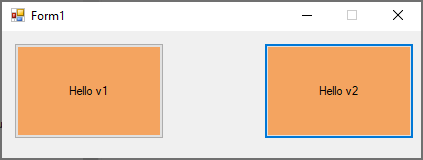
\includegraphics[scale=0.6]{images/exp-v3.png}
    \captionof{figure}{Version 3 of the experiment application}\label{fig:exp-v3}
    \endgroup
\end{tabularx}


However, a different result is displayed when using 'widget title' and 'widget control type' as widget attributes for the abstract states. Namely, the button with the label 'Hello v1' is removed between the first two versions. The buttons labelled 'Hello v1' and 'Hello v2' are added. Between versions 2 and 3, no differences are observed.

This change difference outcome can be explained by the way the proof of concept is working. The widget tree of version 1 contains one button, whereas the widget tree of version 2 contains two buttons. Therefore both the abstract and the concrete identifiers are different for both widget trees. The proof of concept change detection checks whether the abstract identifier of version 1 can be found in version 2, which it cannot, so the state is marked as removed. The state of version 2 can likewise not be found in version 1 so that state is marked as new.

The chosen widget attributes explain the absence of changes between versions 2 and 3. Neither the title nor the control type has changed. Since those attributes were used for the abstract identifier, TESTAR did not detect a change. 

In section (\ref{research-questions}), the research questions are discussed. Of course, one of the questions will investigate how the change detection algorithm must be implemented. The findings of the two-button app should be considered, and the experiment should be adapted to contain different changes to test on. 

%\newpage
\subsection{TESTAR in containers}
A recent master thesis by Slomp explains how TESTAR can be integrated into a \acrfull{ci} environment \cite{thesisSlomp}. Slomp introduced TESTAR into the world of Docker and container and integrated TESTAR into an Azure DevOps pipeline. A pipeline is a collection of steps that can automatically build, test and release software. A container bundles all the software, configuration files and libraries together so that an application can run \cite{ms-container}. 

When TESTAR is being run within the Azure DevOps pipeline, the TESTAR GUI is not shown. Running TESTAR is not a problem. However, to analyse the outcome of TESTAR, the users need to install TESTAR and have access to the OrientDb database location. 

By moving the code for change detection and visualisation into a stand-alone web application, the user can analyse the outcome on their browser. Since TESTAR is wrapped into a container, the stand-alone tool will also be wrapped to provide the same infrastructure. Nevertheless, it is up to the IT administrator how they deploy the TESTAR suite. 

Additionally, to the user's benefit, a TESTAR developer can also benefit from the application's separation. Changes to either the separate application or TESTAR can be made without being conflicting with the other. Each tool can focus on one goal, while TESTAR can focus on testing GUI applications. 
    \newpage

    \chapter{Research} \label{questions}
In this chapter, the research questions for the thesis are formulated. What research method will be used, and how the questions are being validated.

\section{Context}
The graduation assignment evolves around change detection and visualising the changes. The result is an external application that connects to OrientDB and calculates and shows the changes. The external application will be built outside \testar. The code created by Pastor Ricós and by Mulders will be used as a starting point for the external application. 

Because change detection is the subject for this graduation assignment, it is assumed that the inferred model generator will generate useful models for change detection. Although the inferred model generator is out-of-scope, it is not ruled out that changes are necessary.

Any automatic learning capabilities are also out-of-scope. A change detection learning capability could be a topic for a future research proposal. Regarding this research proposal, a human will be needed to evaluate the results and outcome of the change detection application.

\section{Research questions} \label{research-questions}
        
The main research question is: \textbf{How can an automated comparison of inferred models help testers finding bugs?}

The main research question is divided into three parts. The first part (\ref{rq:detect-changes}) will research how to detect changes between different versions of the same GUI software (SUT) \cite{testar-todo}. The second part (\ref{rq:diff-visualisation}) will research how to visualise the detected changes. A third Research Question \ref{rq:validation} is dedicated to validating the previous research questions. The research questions are as follows: 

\begin{questions}
    \item How to detect changes between two versions of the SUT? \label{rq:detect-changes}
    \begin{questions}
        \item What is change detection, and what do we want to use it for? \label{rq:what-is-change-detection}
        \item Which properties make a model useful for change detection? \label{rq:useful-detection}
        \item Which \testar configuration will generate the useful model? \label{rq:testar-config}
        \item How can we find changes between two models? \label{rq:finding-changes}
    \end{questions}

    \item How to visualise the detected differences to the user? \label{rq:diff-visualisation}
    \begin{questions}
        \item What tooling is available to show the result of the change detection? \label{rq:tooling}
        \item How to visualise each change? \label{rq:type-visualisation}
        \item How to generate the shortest set of actions that helps the user to reach the changed state in the SUT? \label{rq:shortest-set}    
    \end{questions}
    
    \item How to validate the results of \ref{rq:detect-changes} and \ref{rq:diff-visualisation}? \label{rq:validation}
    \begin{questions}
        \item What are the requirements for validation applications? \label{rq:req-apps}
        \item Which applications can be used for validation? \label{rq:validation-apps}
    \end{questions}
\end{questions}

\subsection{\ref{rq:what-is-change-detection} What is change-detection, and what do we want to use it for?}
To get an answer for \ref{rq:what-is-change-detection}, a literature study will be conducted. The literature study aims to bring an overview of change detection in general and its application in the \testar context. Not only change detection in the GUI but also other change detection methods in the field of Software Engineering, like cross-browser testing. 

\subsection{\ref{rq:useful-detection} Which properties make a model useful for change detection?}
The outcome of \ref{rq:useful-detection} is a list of requirements for the inferred model that are needed to enable change detection. For example, can a non-deterministic state model be used? However, it also includes requirements for the algorithm, like, what are acceptable calculation speeds and how big can a state model be while still complying with the speed requirement? When the set of properties are known, Vaandrager's criteria are used to validate the model \cite{vaandrager}.

\subsection{\ref{rq:testar-config} Which \testar configuration will generate a useful model?}
There are a couple of ways to change the outcome of an inferred model, for example, picking widget attributes for the hash calculation. These configurations can influence the usefulness of the model. The outcome of \ref{rq:useful-detection} should result in a \testar configuration file that configures \testar to generate this useful model. It might be necessary to make code changes in the state model generation or to the identification calculation to implement a Merkle tree approach. Using a Merkle tree could help with comparison to graphs, especially changed in the widget tree. 

A threat of validity for \ref{rq:testar-config} is that every application under test needs its unique configuration. Therefore, it might be wise to look into all widgets attributes during the change detection and not take the hash of a state for the comparison. The configuration can be used for tuning the model and the change detection by taking the above approach.

\subsection{\ref{rq:finding-changes} How can we find changes between two models?}
\ref{rq:finding-changes} is the closing question in which the algorithm is coded in Java. In a recent master thesis by Slomp \cite{thesisSlomp}, it is possible to run \testar in a Docker container. As a consequence, \testar can run without a GUI. Therefore the change detection algorithm will run in a separate application, outside the \testar context. The result of the change detection needs to be saved to a data store, preferably the already existing OrientDb database. 

\subsection{\ref{rq:tooling} What tooling is available to show the detected differences?}
Aside from the inferred model, Mulders also created an application to visualise the models. It is essential to state that Mulders did extensive research on which technology fits his needs best. \ref{rq:tooling} will look at the results of Mulders and revalidate whether the libraries are suitable for visualising the differences. 

\subsection{\ref{rq:type-visualisation} How to visualise change?}
\ref{rq:type-visualisation} will look into the execution of the visualisation tool. How can added, removed or altered states in the inferred model be visualised the best? Like \ref{rq:finding-changes} this also includes moving the visualisation tool into its separate application, outside the \testar context. The requirements and GUI proposals will be discussed with the \testar stakeholders. 

\subsection{\ref{rq:shortest-set} How to generate the shortest set of actions that helps the user to reach the changed state in the SUT?}
One of the requirements of the visualisation is showing how to reach the state that has changed. Dijkstra's algorithm \cite{dijkstra1959note} is a well-known algorithm to find the shortest path for a given graph. However, as Goldberg and Harrelson \cite{goldberg2005computing} showed, it is not the most optimal shortest path algorithm, especially with massive graphs. 

\subsection{\ref{rq:req-apps} What are the requirements for validation applications?}
To validate the outcome of the change detection algorithm, we will need to have an application to test it on. The research question will create a set of requirements for the validation application, like multiple versions. The set will be discussed with the supervisors to make sure nothing will be forgotten.

\subsection{\ref{rq:validation-apps} Which applications can be used for validation?}
During development and system testing, the two-button app will be extended and used. Although the app is excellent during the development phase, it is nowhere close to a real-world application. Based on the outcome of \ref{rq:req-apps}, an application needs to be found in order to test the change detection algorithm.

In addition to the application found, F-secure will be asked for feedback on the algorithm and the visualisation. F-Secure is a company based in Finland that provides security solutions to its customers and are currently testing the proof of concept of Pastor Ricós \cite{f-secure}.

With the combination of real-world application and the feedback from F-Secure, biased towards a single point of view for the algorithm will be minimized. 
    \newpage    
    
    \chapter{Research results}

This chapter is devoted to the research results. For each research question, a separate section is used. 

\section{\ref{rq:what-is-change-detection} What is change-detection, and what do we want to use it for?}

\subsection{What is change?} \label{what-is-change}

Not many research papers could be found that define the word change. A clear definition of the word change can be found in a psychology paper by Rensink \cite{rensink2002change}.

\begin{quote}
    "The word change generally refers to a transformation or modification of something over time. As such, this notion presumes a nonchanging substrate on which changes are imposed. More precisely, change is defined here [the paper] as the transformation over time of a well-defined, enduring structure." (Rensink, 2002, p. 248).
\end{quote}

The definition of the word change can be translated to the language of \testar. The "well-defined, enduring structure" refers to the GUI of the system under test, whereas the "transformation over time" refers to the various version of the SUT. The "something" refers to a part of the GUI that can change like: Widget tree, the state or an action. 

Besides defining the word change, Rensink also describes the differences between changes and differences. A change is a transformation of the same 'something', whether a difference lacks the property of the same something. For example, what are the differences between two distinct SUT, or the same SUT but in two distinct environments or Internet Browsers? A limit to the change detection algorithm is that the SUT needs to be executed in the same environment; otherwise, false-positive changes can occur.

This distinction of definitions between change and differences give the first limit to this research paper's proposed change detection algorithm. The change detection algorithm will give the changes of a SUT, between versions, in the same environment since a different environment can influence the model and therefore influence the outcome of the change detection.

\subsection{What change detection?}

toool made by F-secure. collaboration with Pekka GUI Driver. both had features. 

automated masking abstract away know a lot. image comparison. 

GUITAR, something. 

F-secure change detection point it own 
new tool, no paper. 

Change what we are intresing in.

starting state depends on existng data. external changes removed. 

percent of change pixel could indicate .... div > 50\% change then different. 
1 level-> differences on the screen.
2 level-> change in the model (state graph)
3 level-> Form testing, from testing correct and incorrect form
 - hint faker library phone number etc...
 - relationship between 

find values on the new page. releation input value and one of the screen. you input phonenumber. on screen is presented on

metaphorfic testing (relationships). 

Alexander Pretengkro finding state machine. (Aho can connect).

Anomoli detection for change. most change happen on one stap. What if the it stop changes Trent, history change some... change on change detection. 
 
 source: meeting 2 dec with IVVES 
 
\section{\ref{rq:useful-detection} Which properties make a model useful for change detection?}
\section{\ref{rq:testar-config} Which \testar configuration will generate a useful model?}
\section{\ref{rq:finding-changes} How can we find changes between two models?}

Abstract Graph comparison
First the software create a ComparableGraph. A Comparable graph only contacts the nodes and edges from the abstract states and abstract actions. The data however will include data from the concrete states and actions. 

When we have a changed abstractstate, get a widgettree of one concrete state
https://www.xmlunit.org/  have a package for both java as .NET to create differences between version.

using a fast mode
the fast mode will only look into changes on the abstract level. Changes like different colours for example




\section{\ref{rq:tooling} What tooling is available to show the detected differences?}

The solution is written outside the \testar application. Doing so makes it possible to work without the context and dependencies of \testar and allows the application to be written in a language more known by the developer. Building the application outside the \testar scope was possible because it only needed the state model data from the OrientDB graph database.

The solution is divided into two major parts. A \testar .NET server and a \testar .NET UI. As the name suggests, they are built and created in the Framework from Microsoft: .NET Core (version 6) \footnote{\url{https://dot.net}}. .NET is an open-source, cross-platform framework. An application created with .NET will run on Windows, Linux and macOS. 

\begingroup
\captionsetup{type=figure}
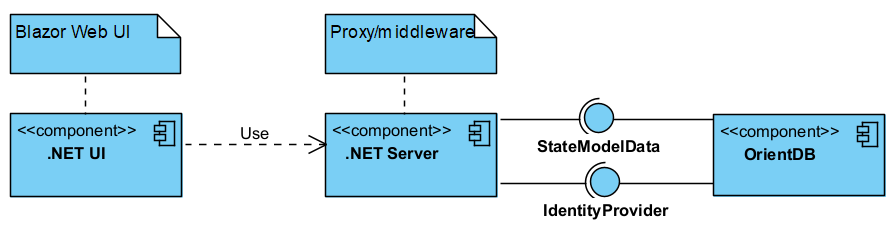
\includegraphics[scale=0.7]{thesis/images/server-ui-comp.png}
\captionof{figure}{.NET UI - Server and OrientDb component model}\label{fig:components}
\endgroup

Figure \ref{fig:components} shows the three components making up the system. The state model data that \testar generated is saved into the OrientDB graph database, the same database used by the .NET server. The .NET UI connects to the .NET server. In the following sections, the different components are explained. 

\subsection{OrientDB Component}
OrientDB is the data storage for \testar. The created application presents the data to the user. In order to query the data, the \textsc{rest} endpoint of OrientDB is used. A \textsc{post} is sent to OrientDB with the query and parameters in the body of the request. An example of the body is displayed in listing \ref{code:example-body}.

\begin{lstlisting}[language=xml, caption=Get AbstractStateModel by the model identifier, label=code:example-body]
{
  "command": "SELECT FROM AbstractStateModel WHERE modelIdentifier = :id",
  "parameters": {
    "id": "1chdi5230521708089"
  }
}
\end{lstlisting}

An alternative way of querying the data is to use the Query \textsc{get} operation. While it is an easy way to query the data it is vanurable to SQL injection since the paramaters are directly used in the URL and can therefor be altered.

The current solution in which the queries are send from the UI to the .NET server is not completely fool proof either. It is still possible to, for example by using the Burp Suite, to alter the \textsc{post} message body and attach the OrientDB server. To circumvent this issue it would be recommended to setup a \textsc{rest} endpoints that returns data and lets the .NET server creates the SQL calls to OrientDB. 

It is not recommended to expose the OrientDB database directly to a public network \cite{orientdb-security}. To build the application with good security in mind, the database is exposed through a Proxy/middle-ware component, the .NET server. In the next section the .NET server component is explained in more detail.

\subsection{.NET Server}

The .NET Server servers as Proxy between the .NET UI component and the already existing OrientDB graph database. The only user of the .NET server is UI component. However it is possible to have other applications use to .NET Server to query data stored in OrientDB. 

The need for the .NET Server was due to browser restrictions and limitations accesing the Database. Two issues arise when the UI was trying to connect to the Database. The issue was \acrfull{cors} and it a security feature in which the server can permit or denay a request from a client if the request was not made by a trusted source \cite{cors}. By default OrientDB does not permit other websites to use the \textsc{rest} endpoints from OrientDB \cite{orientdb-webserver}. It is possible to enable to CORS in the OrientDB configuration but that would mean administrators should edit the OrientDB config before the .NET application could be used and secondly it would not fix the second issue, accessing the session cookie.

The second issue prevented the UI to read the cookie created by OrientDB. Before a user can query the data it need to sign in the OrientDB. This is accounplised by executing a \textsc{get} command to the /connect/database endpoint and provide the username and password, encoded with the base64 algorithm, as a authentication header. If the credentials are valid, the OrientDB will return a \textsc{204 ok} response with a \textsc{osessionid} in the response headers. The \textsc{osessionid} is used to authenticate the user on future calls.

It was impossible to retrieve the \textsc{osessionid} and reuse it in the data retrieval processes. Not able to save the \textsc{osessionid} resulted in saving the username and password in local storage of the browser, making it available for retrieval with a Cross Site Scripting attack. 

database need to be provided in the configuration. Based on user feedback it also possible to enable multi database command. With that feature -> user can access multiple database by providing database name before username 

is signed by the sever. 

In Addition to data is user identies also stored in the OrientDB database. 

\subsection{.NET UI}
The .NET UI component is created in Blazor. Blazor is an interactive web UI technology that allows running .NET code in the browser \cite{what-is-blazor}. For the graphical layer, Blazor uses HTML. The Blazor application runs in a browser, which can provide the user with all kinds of tools for troubleshooting. Bootstrap is used as a front-end framework \footnote{\url{https://getbootstrap.com}}.

Instead of writing the application code in Javascript, Blazor uses C\# and the .NET Core framework, although it is still possible to use existing Javascript libraries. For example, the state model visualisation engine, Cytoscape, is moved from the \testar analysis engine to the new \testarnet UI.

Since both the server and the UI are running C\# code, it is possible to share the core application code in both projects. As a side benefit, the core application code can be reused in smaller applications dedicated to a single task, like change detection. 

The UI component needs to be hosted on a web server that can host static files. Blazor is interactive by nature, but from the server's perspective, is it a static site since it does not have any server-side code execution. All code executions are handled on the user's computer. Before the user can use the website, it is downloaded on its computer before it gets executed. After the download, the application runs on the user's computer and the traffic to and from the .NET server will not travel through the public internet. 

The UI component is publicly available on \url{https://app.testarin.net} (read as \testar in dot net). 

Based on user feedback, a docker container with the UI application is published to the docker hub \footnote{\url{https://hub.docker.com/repository/docker/rneeft/testar-net-ui}}. In the docker container, the Nginx \footnote{\url{https://nginx.org/en/}} web server hosts the static site.

\subsection{Authentication \& Authorisation}
The .NET server helps with solving the security issues but still provide a secure and open authentication endpoint. External applications that want to use the .NET endpoints must first authenticate with the .NET server upon it will return a \acrfull{jwt}. A JWT is defined as a "compact, URL-safe means of representing claims to be transferred between two parties." \cite{jones2015json}.

Before the user can use the UI it needs to authenticate itself. Figure \ref{fig:auth-sd} shows the sequence diagram how the authentication flow is handled. Since the user identities are stored in the identity provider of the graph database, it is important to note that the .NET server does neither handle authentication nor authorisation. As visible in the figure it only provides a sign in proxy and generated a JWT around the oSessionId. The authentication and authorisation is handled by the OrientDB server. When the user provides incorrect credentials, the graph database will return a \verb|401 Unauthorized| and the Server will return that status code to the UI.

\begingroup
\captionsetup{type=figure}
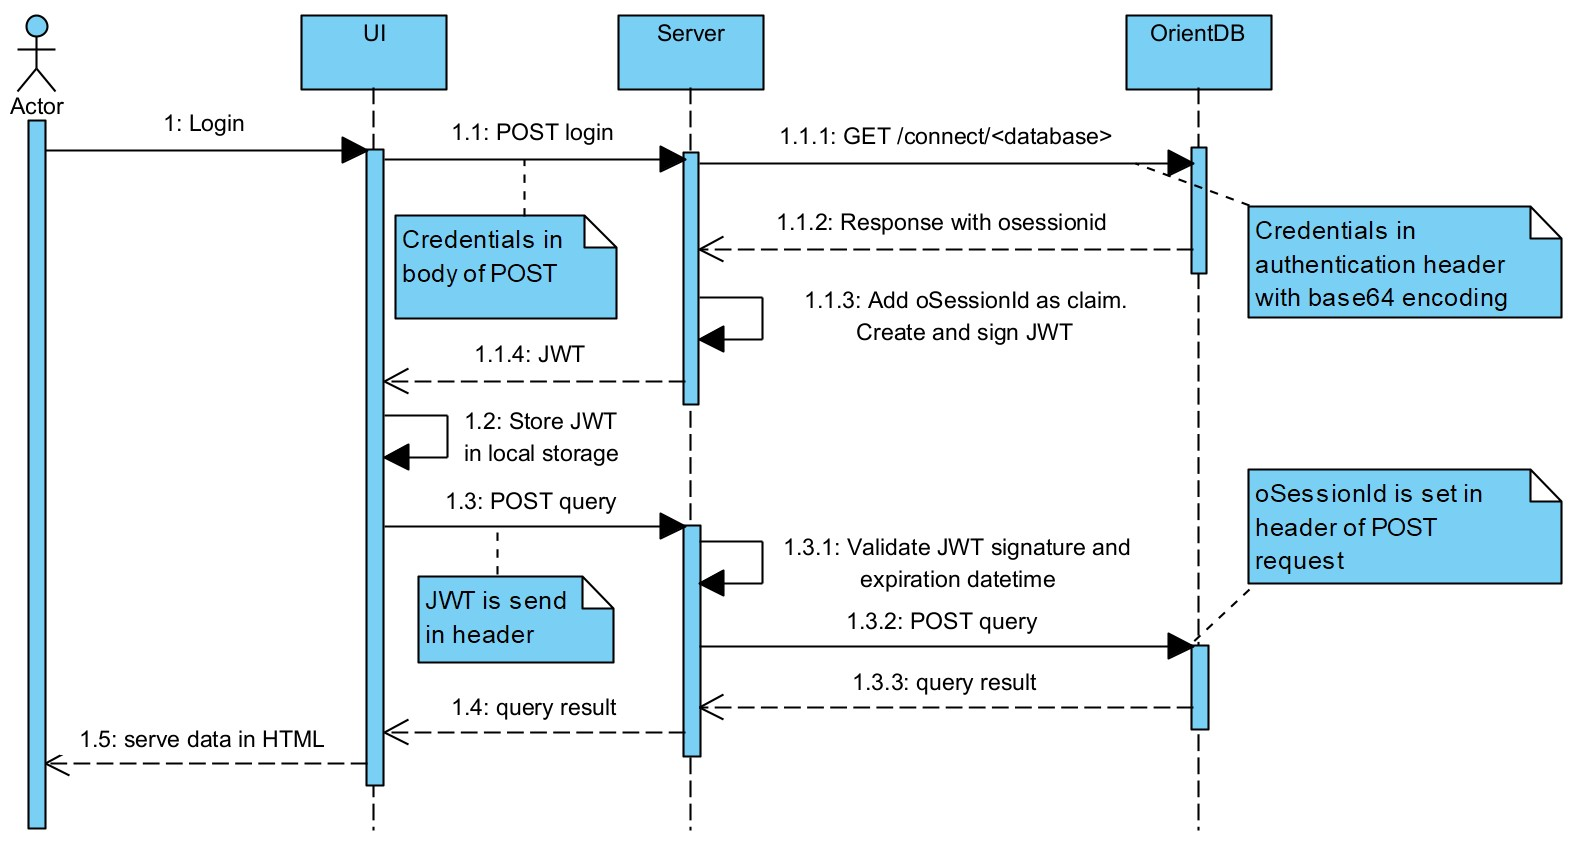
\includegraphics[scale=0.4]{thesis/images/authentication-sd.png}
\captionof{figure}{Authentication sequence (UML 2.0)}\label{fig:auth-sd}
\endgroup

An example of the JWT generated by the server is displayed in listing \ref{code:jwt}. The JWT can be decoded by anyone, for example with a website like \url{https://jwt.io}. The corresponding header and payload is displayed in listing \ref{code:jwt-payload}. In the JWT, two dots are visible which shows the different sections of the token. The first section is dedicated to the header information (lines 1-4 in listing \ref{code:jwt-payload}. The middle section contains the payload (lines 5-12 in listing \ref{code:jwt-payload}). The third and last section contains the signing information. 

\begin{lstlisting}[language=xml, caption=Example JSON Web Token (line breaks for display purposes only), style=nonrstyle, label=code:jwt]
eyJhbGciOiJIUzI1NiIsInR5cCI6IkpXVCJ9.eyJodHRwOi8v
c2NoZW1hcy54bWxzb2FwLm9yZy93cy8yMDA1LzA1L2lkZW50a
XR5L2NsYWltcy9uYW1lIjoidGVzdGFyIiwiT3JpZW50RGJTZX
NzaW9uIjoiT1NFU1NJT05JRD1PUzE2NDk3OTY5OTgxODgtMTE
3NTE5OTcxMDIyNDcxNTA0MyIsIkRhdGFiYXNlTmFtZSI6InRl
c3RhcjIiLCJleHAiOjE2NDk4MDA1OTgsImlzcyI6Imh0dHA6L
y9sb2NhbGhvc3QiLCJhdWQiOiJodHRwOi8vbG9jYWxob3N0In
0.zkSDTOuNrn9lR0ca6JLQsbSiLEskEBC_uY937q9sSU0
\end{lstlisting}

Every JWT is signed by the server (see the self-message 1.1.3 in figure \ref{fig:auth-sd}) with a secret provided during the startup of the .NET Server. With the signing information, the server can validated that it generated the JWT and that it is safe to assume the information in the payload is legit. 

There are a couple of intresting claims visible when viewing the payload. exp... by default 5 minutes. same lenght as the orientDB cookie lifetime. Line \verb|6| shows the username of the user. Line \verb|7| shows the OrientDbSession which the .NET server is using to communicate to the graph database. Line \verb|8| displayed the databasename. The databasename is only visible when on the server the feature 'MultipleDatabases' is activated. Lines \verb|9| (exp), \verb|10| (iss) and \verb|11| (aud) are showing the claims registered in the \acrfull{iana} \cite{jones2015json}. \verb|exp| Stands for 'expiration' and shows the expiration time in seconds (in Unix epoch). By default the expiration time set to 5 minutes, which is the same as the orientdb session id. 




since jwt is signed with a secret only known by the server, the server can validate whether it generated the JWT.

\begin{lstlisting}[language=xml, caption=Decoded JWT header and Payload of the JWT given in listing \ref{code:jwt}, label=code:jwt-payload]
{
  "alg": "HS256",
  "typ": "JWT"
}
{
  "http://schemas.xmlsoap.org/ws/2005/05/identity/claims/name": "testar",
  "OrientDbSession": "OSESSIONID=OS1649796998188-1175199710224715043",
  "DatabaseName": "testar2",
  "exp": 1649800598,
  "iss": "http://localhost",
  "aud": "http://localhost"
}
\end{lstlisting}






\subsubsection{Hosting the application}
In section \ref{sec:testar-in-docker} is indicated that \testar is running in a docker container. The new .NET components are also published as docker containers. 


For all applications, a docker image is created. 





Blazor

two second
Testar server
security
proxy , 
image
Testar UI

docker image

\section{\ref{rq:type-visualisation} How to visualise change?}

merge graph \cite{andrews2009visual}
the graph needs to be similar are "enough"

\section{\ref{rq:shortest-set} How to generate the shortest set of actions that helps the user to reach the changed state in the SUT?}

\section{\ref{rq:req-apps} What are the requirements for validation applications?}

\section{\ref{rq:validation-apps} Which applications can be used for validation?}

    \newpage    
    
    % Reference list
    % keep using the alpha style, this makes it easier for the reader to correlate the used citations
    \bibliographystyle{alpha}
    \bibliography{bibliography}
    
    % List of abbreviations
    
    
    % Appendices

\end{document}